\section{Monday, July 18, 2022}

\subsection{Independence}

Let $A$ and $B$ be events such that $P(A) = P(A|B)$. By definition, $A$ and $B$ are \vocab{independent}. This means that knowing whether or not $B$ occurs does not change $P(A)$. In other words, $B$ provides no information about $A$.

An equivalent definition of independence is $$P(A \cap B) = P(A) \times P(B).$$

It follows that if $A$ is independent of $B$, then $B$ is independent of $A$: $P(B|A) = P(B)$. In experiments with multiple trials, experimenters try to conduct independent trials so that no one trial can affect any other.

Some examples include \textit{sampling} from an urn with replacement, or some \textit{gambles} like coin tossing, roulette, or dice. \textit{Card games} include poker or bridge, where each round is independent of the others as long as the deck is thoroughly shuffled between rounds. Blackjack or twenty-one does not have independent rounds because the deck is not shuffled between rounds. (The ``deck" is actually 8 decks of 52 cards). Generally, sampling relatively few items from a large population yields approximate independence.

\subsection{Mutual and Pairwise Independence}
We can extend independence from a pair of events to a collection of events.

Let $A_{1}, A_{2}, \ldots, \A_{n}$ be events such that $$P(A_{i}) \cap A_{j}) = P(A_{i}) \times P(A_{j}) \, \text{for} \, i \neq j$$
$$P(A_{i}) \cap A_{j} \cap A_{k}) = P(A_{i}) \times P(A_{j}) \times P(A_{k}) \, \text{for distinct} \, i, j, k$$
$$\cdots$$
$$P(A_{1}) \cap \cdots A_{n} = P(A_{1}) \times P(A_{2}) \cdots P(A_{n})$$
Equivalently, for any $k$ events $A_{i}_{1}, A_{i}_{2}, \ldots, A_{i}_{k}$ we have $$P(A_{i}_{1}) \cap \cdots \cap A_{i}_{k} = P(A_{i}_{1}) \times P(A_{i}_{2}) \times \cdots \times P(A_{i}_{k}).$$

If these formulas are true, then $A_{1}, A_{2}, \ldots, A_{n}$ are \vocab{mutually independent}. We usually just say that the events are \vocab{independent}. The intersection of two events (and all possible pairs of events from $A_{i}$ to $A_{n}$) is their product. Then, picking any subsets of events, their intersection probability is also the product of unconditional probabilities.

The definition of mutual independence involves $2^{n}-n-1$ conditions. It's natural to wonder if the definition can be simplified. $A_{1}, A_{2}, \ldots, A_{n}$ are \vocab{pairwise independent} if $$P(A_{i}) \cap A_{j} = P(A_{i}) \times P(A_{j}) \, \text{for} \, i  \neq j.$$ This is not the same as mutual independence as shown below.

\textbf{Example 1}: Suppose a fair coin is tossed twice. Then $S=\{HH, HT, TH, TT\}$. The outcomes are equally likely. Define $A = \{HH, HT\}$, $B = \{HH, TH\}$, and $C = \{HH, TT\}$.

Each of these three events has probability $1/2$ and they are pairwise independent. (Check!) But, $P(A \cap B \cap C) = 1/4 \neq P(A) \times P(B) \times P(C)$ so these events are not mutually independent.

\subsection{Multiplication Rule and Independence}
If $A$ and $B$ are independent, by definition $P(A \cap B) = P(A) \times P(B)$. The multiplication rule extends to several independent events, according to the definition of (mutual) independence.

It's easy to see that if $A$ and $B$ are independent, so are $A^\mathsf{'}$ and $B$, $A$ and $B^\mathsf{'}$, and $A^\mathsf{'}$ and $B^\mathsf{'}$.

Good experimental practice calls for repeated trials, measurements, etc., which must be conducted so that one trial cannot affect results of others. This means the trials are independent.

\subsection{Bernoulli Trials}

An important class of applications involves mutually independent trials resulting in either ``success" or ``failure". If each trial has the same success probability $p$, then $P(n \text{successes} = p^n$ and $P(n \text{failures}) = (1-p)^n$. Such trials are called \vocab{Bernoulli Trials}.

More generally, the probability of each sequence of trials with $k$ successes if $p^k(1-p)^{n-k}$. This probability does not depend on the ordering of successes and failures.
t
% When Bernoulli trials are being conducted, we are not so much interested in a probability of a single outcome of $n$ Bernoulli outcomes. If we run a trial with $n=10$, there are 1024 outcomes. However, we'd like to know something more reasonable: ``what is the probability of $k$ successes out of order?"

Usually, the probability of a specific sequence of successes and failures is not important. Instead, we want a formula for $P(\text{exactly} \, k \, \text{successes})$.

Since all sequences with $k$ successes have common probability $p^k(1-p)^{n-k}$, we only have to count those sequences. The successful trials are a combination of $k$ trials from a set of $n$ trials, so the count is $n \choose k$. Therefore, $$P(k \, \text{successes in} \, n \, \text{trials}) = {n \choose k} p^k(1-p)^{n-k}.$$ This is the \vocab{binomial probability} formula. An example of an application includes inspecting a parallel system to find out how many of the trials are successes. 

\textbf{Example 2}: Application - Systems of Independent Components: Complex systems can fail if some critical component fails. Assume components work or fail independently of one another. First, we consider a \textit{series system} (see image below). 

The components work independently with probability $p_{j}, j=1, 2, 3$. If any component fails, the system will fail. The probability that the system works is $P(\text{system works}) = p_{1} \times p_{2} \times p_{3}$.

If possible, redundancy is built into a complex system such that a single subsystem's failure will not cause the whole system to fail. An example is using a parallel system instead of a series system (see image below). Again, assume there are three independent components as above. The system works unless all of its components fail. Hence, $P(\text{system works}) = 1-P(\text{system fails}) = 1-(1-p_{1}) \times (1-p_{2}) \times (1-p_{3})$. We subtract the failure probabilities from 1.

\vspace{0in}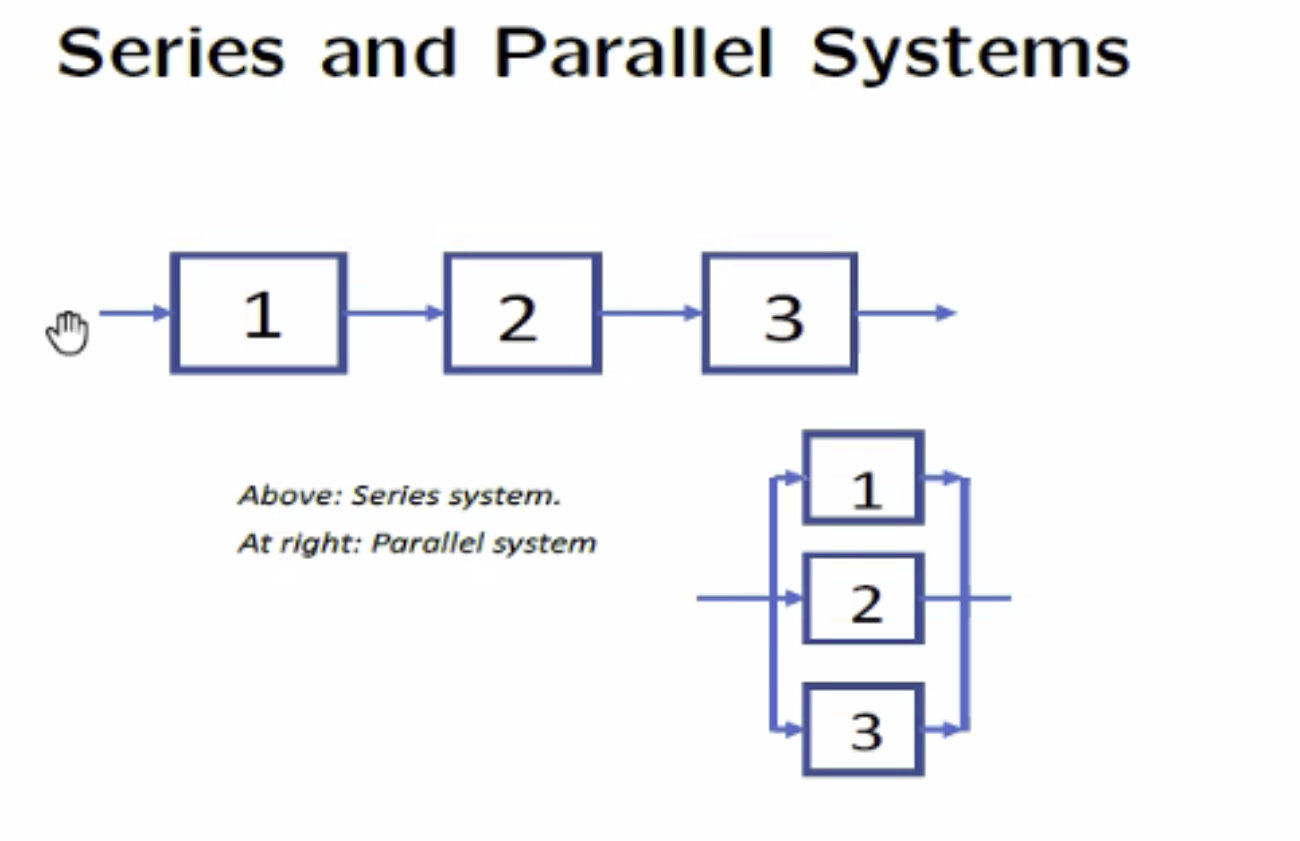
\includegraphics[scale=0.4]{media/wk2systems.png} \\